\begin{table*}[t!]
\begin{center}
\setlength{\tabcolsep}{5pt}
\renewcommand{\arraystretch}{1.1}
\small
\begin{tabular}{l|rrrr|rrrr|rrrr}
  & \multicolumn{4}{c|}{\Sm} & \multicolumn{4}{c|}{\Med} & \multicolumn{4}{c}{\Lg}  \\
\hline
multi-task training? &
&
\checkmark &
&
\checkmark &
&
\checkmark &
&
\checkmark &
&
\checkmark &
&
\checkmark
\\
stage-wise training? &
 &
 &
\checkmark &
&
 &
 &
\checkmark &
&
 &
 &
\checkmark &
\\
test-time bbox reg? & & & \checkmark & \checkmark & & & \checkmark & \checkmark & & & \checkmark & \checkmark \\
VOC07 mAP & 52.2 & 53.3 & 54.6 & \bf{57.1} & 54.7 & 55.5 & 56.6 & \bf{59.2} & 62.6 & 63.4 & 64.0 & \bf{66.9} \\
\end{tabular}
\end{center}
\caption{Multi-task training (forth column per group) improves mAP over piecewise training (third column per group).}
\tablelabel{multitask}
\vspace{-0.5em}
\end{table*}

\section{Design evaluation}

We conducted experiments to understand how Fast R-CNN compares to R-CNN and SPPnet, as well as to evaluate design decisions.
Following best practices, we performed these experiments on the PASCAL VOC07 dataset.
%Based on those results, we train and test a couple of models on VOC12.

\subsection{Does multi-task training help?}
\seclabel{multitask}
Multi-task training is convenient because it avoids managing a pipeline of sequentially-trained tasks.
But it also has the potential to improve results because the tasks influence each other through a shared representation (the ConvNet) \cite{caruana1997multitask}.
Does multi-task training improve object detection accuracy in Fast R-CNN?

To test this question, we train baseline networks that use only the classification loss, $L_\textrm{cls}$, in \eqref{loss} (\ie, setting $\lambda = 0$).
These baselines are printed for models \Sm, \Med, and \Lg in the first column of each group in \tableref{multitask}.
Note that these models \emph{do not} have bounding-box regressors.
Next (second column per group), we take networks that were trained with the multi-task loss (\eqref{loss}, $\lambda = 1$), but we \emph{disable} bounding-box regression at test time.
This isolates the networks' classification accuracy and allows an apples-to-apples comparison with the baseline networks.
%(Results with bounding-box regression are shown in the third column, per group, to illustrate its effect.)

Across all three networks we observe that multi-task training improves pure classification accuracy relative to training for classification alone.
The improvement ranges from $+0.8$ to $+1.1$ mAP points, showing a consistent positive effect from multi-task learning.

Finally, we take the baseline models (trained with only the classification loss), tack on the bounding-box regression layer, and train them with $L_{loc}$ while keeping all other network parameters frozen.
The third column in each group shows the results of this \emph{stage-wise} training scheme: mAP improves over column one, but stage-wise training underperforms multi-task training (forth column per group).

\subsection{Scale invariance: to brute force or finesse?}
\seclabel{scale}
We compare two strategies for achieving scale-invariant object detection: brute-force learning (single scale) and image pyramids (multi-scale).
In either case, we define the scale $s$ of an image to be the length of its \emph{shortest} side.

All single-scale experiments use $s = 600$ pixels;
$s$ may be less than $600$ for some images as we cap the longest image side at $1000$ pixels and maintain the image's aspect ratio.
These values were selected so that \vggsixteen fits in GPU memory during fine-tuning.
The smaller models are not memory bound and can benefit from larger values of $s$; however, optimizing $s$ for each model is not our main concern.
We note that PASCAL images are $384 \times 473$ pixels on average and thus the single-scale setting typically upsamples images by a factor of 1.6.
The average effective stride at the \roi pooling layer is thus $\approx 10$ pixels.

In the multi-scale setting, we use the same five scales specified in \cite{he2014spp} ($s \in \{480, 576, 688, 864, 1200\}$) to facilitate comparison with SPPnet.
However, we cap the longest side at $2000$ pixels to avoid exceeding GPU memory.

\begin{table}[h!]
\begin{center}
\setlength{\tabcolsep}{4.7pt}
\renewcommand{\arraystretch}{1.1}
\small
\begin{tabular}{l|rr|rr|rr|r}
 & \multicolumn{2}{c|}{SPPnet \ZF}  & \multicolumn{2}{c|}{\Sm} & \multicolumn{2}{c|}{\Med} & \Lg \\
\hline
scales & 1 & 5 & 1 & 5 & 1 & 5 & 1 \\
test rate (s/im) & 0.14 & 0.38 & \bf{0.10} & 0.39 & 0.15 & 0.64 & 0.32 \\
VOC07 mAP & 58.0 & 59.2 & 57.1 & 58.4 & 59.2 & 60.7 & \bf{66.9}
\end{tabular}
\end{center}
\caption{Multi-scale vs. single scale.
SPPnet \ZF (similar to model \Sm) results are from \cite{he2014spp}.
Larger networks with a single-scale offer the best speed / accuracy tradeoff.
(\Lg cannot use multi-scale in our implementation due to GPU memory constraints.)
}
\tablelabel{scales}
\vspace{-0.5em}
\end{table}

\tableref{scales} shows models \Sm and \Med when trained and tested with either one or five scales.
Perhaps the most surprising result in \cite{he2014spp} was that single-scale detection performs almost as well as multi-scale detection.
Our findings confirm their result: deep ConvNets are adept at directly learning scale invariance.
The multi-scale approach offers only a small increase in mAP at a large cost in compute time (\tableref{scales}).
In the case of \vggsixteen (model \Lg), we are limited to using a single scale by implementation details. Yet it achieves a mAP of 66.9\%, which is slightly higher than the 66.0\% reported for R-CNN \cite{rcnn-pami}, even though R-CNN uses ``infinite'' scales in the sense that each proposal is warped to a canonical size.

Since single-scale processing offers the best tradeoff between speed and accuracy, especially for very deep models, all experiments outside of this sub-section use single-scale training and testing with $s = 600$ pixels.

\subsection{Do we need more training data?}
\seclabel{moredata}
A good object detector should improve when supplied with more training data.
Zhu \etal \cite{devaMoreData} found that DPM \cite{lsvm-pami} mAP saturates after only a few hundred to thousand training examples.
Here we augment the VOC07 trainval set with the VOC12 trainval set, roughly tripling the number of images to 16.5k, to evaluate Fast R-CNN.
%\cite{agrawal2014analyzing}.
Enlarging the training set improves mAP on VOC07 test from 66.9\% to 70.0\% (\tableref{voc2007}).
When training on this dataset we use 60k mini-batch iterations instead of 40k.

We perform similar experiments for VOC10 and 2012, for which we construct a dataset of 21.5k images from the union of VOC07 trainval, test, and VOC12 trainval.
When training on this dataset, we use 100k SGD iterations and lower the learning rate by $0.1\times$ each 40k iterations (instead of each 30k).
For VOC10 and 2012, mAP improves from 66.1\% to 68.8\% and from 65.7\% to 68.4\%, respectively.
%Fast R-CNN accuracy should improve if more training data become available.

\subsection{Do SVMs outperform softmax?}
Fast R-CNN uses the softmax classifier learnt during fine-tuning instead of training one-vs-rest linear SVMs post-hoc, as was done in R-CNN and SPPnet.
To understand the impact of this choice, we implemented post-hoc SVM training with hard negative mining in Fast R-CNN.
We use the same training algorithm and hyper-parameters as in R-CNN.
\begin{table}[h!]
\begin{center}
\setlength{\tabcolsep}{6pt}
\renewcommand{\arraystretch}{1.1}
\small
\begin{tabular}{l|l|r|r|r}
  method & classifier & \Sm & \Med & \Lg \\
\hline
R-CNN \cite{girshick2014rcnn,rcnn-pami} & SVM & \bf{58.5} & \bf{60.2} & 66.0 \\
\hline
FRCN [ours] & SVM & 56.3 & 58.7 & 66.8 \\
FRCN [ours] & softmax & 57.1 & 59.2 & \bf{66.9} \\
\end{tabular}
\end{center}
\caption{Fast R-CNN with softmax vs. SVM (VOC07 mAP).}
\tablelabel{svm}
\vspace{-0.5em}
\end{table}

\tableref{svm} shows softmax slightly outperforming SVM for all three networks, by $+0.1$ to $+0.8$ mAP points.
This effect is small, but it demonstrates that ``one-shot'' fine-tuning is sufficient compared to previous multi-stage training approaches.
We note that softmax, unlike one-vs-rest SVMs, introduces competition between classes when scoring a \roi.

\subsection{Are more proposals always better?}

%Fast R-CNN enables researchers to test ideas that would have been prohibitively slow in the past.
%For example, we can study the behavior of Fast R-CNN when using a large number of object proposals.

There are (broadly) two types of object detectors: those that use a \emph{sparse} set of object proposals (\eg, selective search \cite{UijlingsIJCV2013}) and those that use a \emph{dense} set (\eg, DPM \cite{lsvm-pami}).
Classifying sparse proposals is a type of \emph{cascade} \cite{Viola01} in which the proposal mechanism first rejects a vast number of candidates leaving the classifier with a small set to evaluate.
This cascade improves detection accuracy when applied to DPM detections \cite{UijlingsIJCV2013}.
We find evidence that the proposal-classifier cascade also improves Fast R-CNN accuracy.

%\paragraph{More sparse proposals.}
Using selective search's \emph{quality mode}, we sweep from 1k to 10k proposals per image, each time \emph{re-training} and \emph{re-testing} model \Med.
If proposals serve a purely computational role, increasing the number of proposals per image should not harm mAP.
\begin{figure}[h!]
\centering
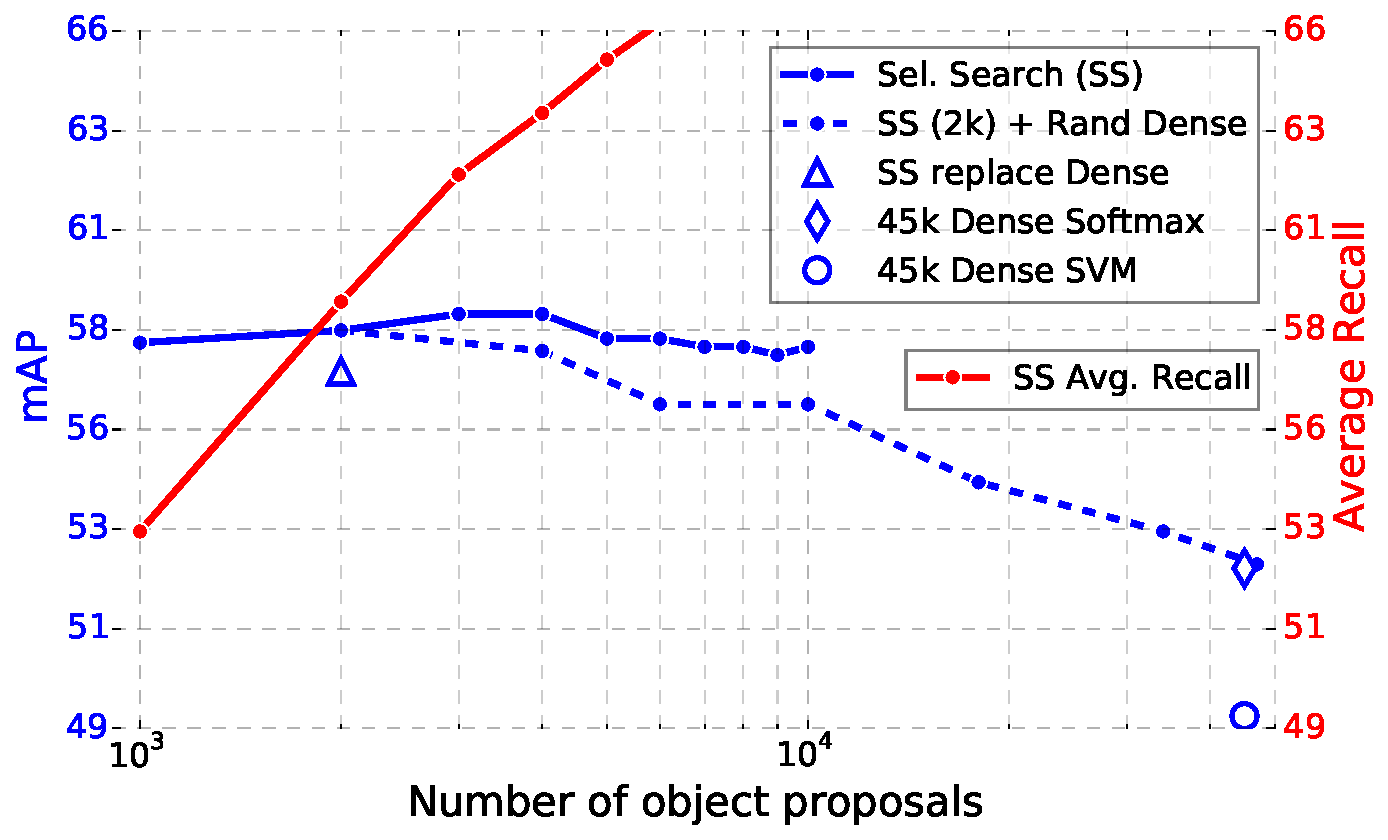
\includegraphics[width=1\linewidth,trim=0em 0em 0 0, clip]{figs/proposals.pdf}
%\vspace{-1em}
\caption{VOC07 test mAP and AR for various proposal schemes.}
\figlabel{proposals}
\end{figure}

We find that  mAP rises and then falls slightly as the proposal count increases (\figref{proposals}, solid blue line).
This experiment shows that swamping the deep classifier with more proposals does not help, and even slightly hurts, accuracy.

This result is difficult to predict without actually running the experiment.
The state-of-the-art for measuring object proposal quality is Average Recall (AR) \cite{Hosang15proposals}.
AR correlates well with mAP for several proposal methods using R-CNN, \emph{when using a fixed number of proposals per image}.
\figref{proposals} shows that AR (solid red line) does not correlate well with mAP as the number of proposals per image is varied.
AR must be used with care; higher AR due to more proposals does not imply that mAP will increase.
Fortunately, training and testing with model \Med takes less than 2.5 hours.
Fast R-CNN thus enables efficient, direct evaluation of object proposal mAP, which is preferable to proxy metrics.


%\paragraph{Dense proposals.}
We also investigate Fast R-CNN when using \emph{densely} generated boxes (over scale, position, and aspect ratio), at a rate of about 45k boxes / image.
This dense set is rich enough that when each selective search box is replaced by its closest (in IoU) dense box, mAP drops only 1 point (to 57.7\%, \figref{proposals}, blue triangle).

The statistics of the dense boxes differ from those of selective search boxes.
Starting with 2k selective search boxes, we test mAP when \emph{adding} a random sample of $1000 \times \{2,4,6,8,10,32,45\}$ dense boxes.
For each experiment we re-train and re-test model \Med.
When these dense boxes are added, mAP falls more strongly than when adding more selective search boxes, eventually reaching 53.0\%.

We also train and test Fast R-CNN using \emph{only} dense boxes (45k / image).
This setting yields a mAP of 52.9\% (blue diamond).
Finally, we check if SVMs with hard negative mining are needed to cope with the dense box distribution.
SVMs do even worse: 49.3\% (blue circle).

%\paragraph{Dense vs. sparse.}
%Sparse object proposal methods are currently the speed bottleneck in Fast R-CNN.
%%Selective search takes 2s / image and EdgeBoxes takes 0.2s / image.
%Replacing them with a dense set of ``sliding windows'' is attractive, since it is essentially free.
%Yet, these experiments provide the first evidence that sparse proposals do indeed ``improve detection quality by reducing spurious false positives'' \cite{Hosang15proposals}.

\subsection{Preliminary MS COCO results}
We applied Fast R-CNN (with \vggsixteen) to the MS COCO dataset \cite{coco} to establish a preliminary baseline.
We trained on the 80k image training set for 240k iterations and evaluated on the ``test-dev'' set using the evaluation server.
The PASCAL-style mAP is 35.9\%; the new COCO-style AP, which also averages over IoU thresholds, is 19.7\%.
